\section{Conceitos Gerais. LKC e LKT}

\frame{
	\frametitle{Introdução}
	\begin{block}{Contextualização}
		Um circuito elétrico pode ser composto por várias malhas, constituídas por elementos que geram ou absorvem energia elétrica. Para calcular as tensões e correntes nesses elementos, necessitamos utilizar as Leis de Kirchhoff devido à complexidade do circuito. Para utilizar estas Leis, precisamos destacar trechos nos quais se aplicam propriedades, facilitando o equacionamento.
	\end{block}
}

\frame{
	\frametitle{Conceitos gerais para análise de circuitos}
	\centerline{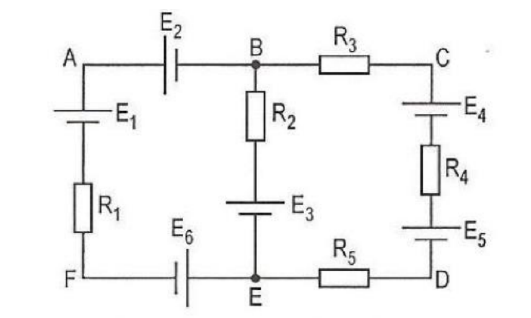
\includegraphics[width=0.5\linewidth]{Figuras/Ch02/fig1.PNG}}
	\begin{block}{Nó}
		Num circuito um \textbf{nó} é qualquer ponto do circuito em que \textbf{três ou mais terminais se liguem}.
		
		\textbf{Obs.:} Alguns autores definem nó como a conexão de \textbf{dois ou mais terminais}. \\
		\begin{itemize}
			\item Neste exemplo, os pontos $B$ e $E$ formam dois nós, em que se interligam geradores e resistores.
		\end{itemize}
	\end{block}
}

\frame{
	\frametitle{Conceitos gerais para análise de circuitos}
	\centerline{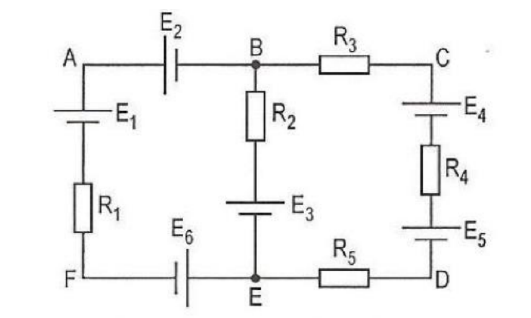
\includegraphics[width=0.5\linewidth]{Figuras/Ch02/fig1.PNG}}
	\begin{block}{Ramo}
		O \textbf{ramo} é o único caminho entre dois nós consecutivos. \\
		\begin{itemize}
			\item Neste exemplo, temos três ramos distintos: o ramo à esquerda composto por $E_6$, $R_1$, $E_1$ e $E_2$, o ramo central composto por $E_3$ e $R_2$ e o ramo à direita, composto por $R_5$, $E_5$, $R_4$, $E_4$ e $R_3$.
		\end{itemize}
	\end{block}
}

\frame{
	\frametitle{Conceitos gerais para análise de circuitos}
	\centerline{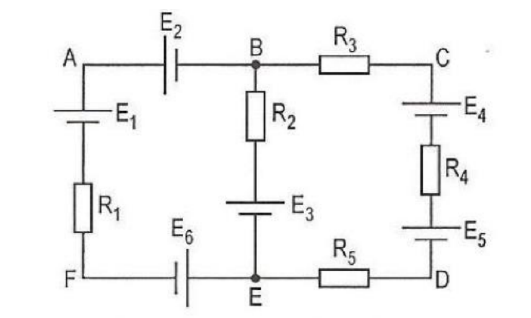
\includegraphics[width=0.5\linewidth]{Figuras/Ch02/fig1.PNG}}
	\begin{block}{Malha}
		Definimos \textbf{malha} como sendo todo circuito fechado constituído por elementos elétricos. \\
		\begin{itemize}
			\item Neste exemplo, notamos que o circuito é composto por três malhas: $ABEF$, $BCDE$ e $ABCDEF$, sendo esta última denominada malha externa.
		\end{itemize}
	\end{block}
}

\frame{
	\frametitle{Leis de Kirchhoff}
	\begin{block}{Introdução}
		A \textbf{Lei de Ohm} por si só não é suficiente para analisar \textbf{circuitos multi-malhas}. Quando unida com as \textbf{Leis de Kirchhoff} formam uma ferramenta poderosa na análise dos circuitos elétricos.
	\end{block}
}

\frame{
	\frametitle{Leis de Kirchhoff}
	\begin{block}{As Leis}
		\begin{enumerate}
			\item 1ª Lei: \textbf{LKC} (Lei de Kirchhoff para Correntes) ou lei dos nós.
			\item 2ª Lei: \textbf{LKT} (Lei de Kirchhoff para Tensões) ou lei das malhas.
		\end{enumerate}
	\end{block}
}

\frame{
	\frametitle{Leis de Kirchhoff - LKC}
	\centerline{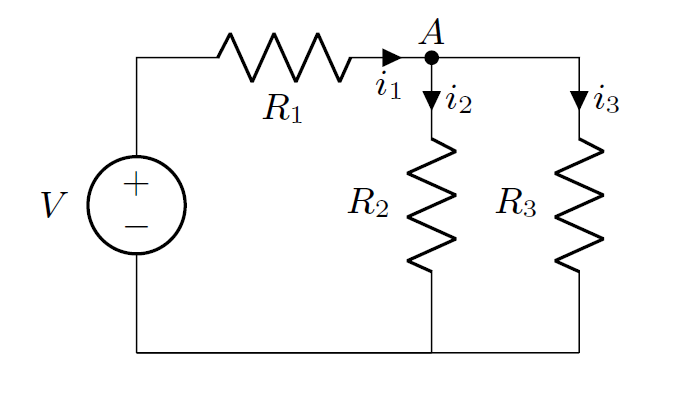
\includegraphics[width=0.6\linewidth]{Figuras/Ch02/fig2.PNG}}
	\begin{block}{Contextualização}
		No nó $A$ entra a corrente total do circuito e do mesmo nó partem as correntes parciais para cada resistor. Como no nó não há possibilidade de armazenamento de cargas ou vazamento das mesmas, tem-se que a \textbf{quantidade de cargas que chegam ao nó é exatamente igual à quantidade de cargas que saem do nó}.
	\end{block}
}

\frame{
	\frametitle{Leis de Kirchhoff - LKC}
	\centerline{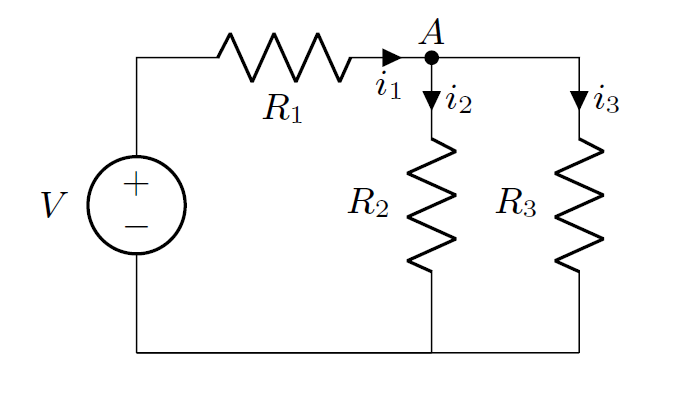
\includegraphics[width=0.6\linewidth]{Figuras/Ch02/fig2.PNG}}
	\begin{block}{Enunciado da 1a Lei de Kirchhoff}
		\textbf{``A soma das correntes que chegam em um nó é sempre igual à soma das correntes que saem deste nó."}
		$$\boxed{\sum_{i=1}^{n} I_{i_{\text{chegam}}} = \sum_{j=1}^{m} I_{j_{\text{saem}}}}$$
	\end{block}
}

\frame{
	\frametitle{Leis de Kirchhoff - LKC}
	\centerline{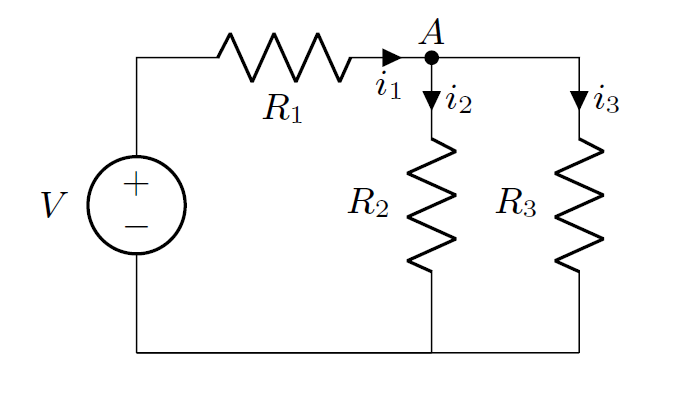
\includegraphics[width=0.5\linewidth]{Figuras/Ch02/fig2.PNG}}
	\begin{block}{Enunciado da 1a Lei de Kirchhoff - alternativo}
		\textbf{``A soma algébrica das correntes que entram e saem de um nó é nula"}. Consideramos que as correntes que \textbf{entram} no nó são \textbf{positivas}, e as que \textbf{saem} são \textbf{negativas}.
		$$\boxed{\sum_{i=1}^{n} I_{i} = 0}$$
	\end{block}
}

\frame{
	\frametitle{Leis de Kirchhoff - LKC}
	\centerline{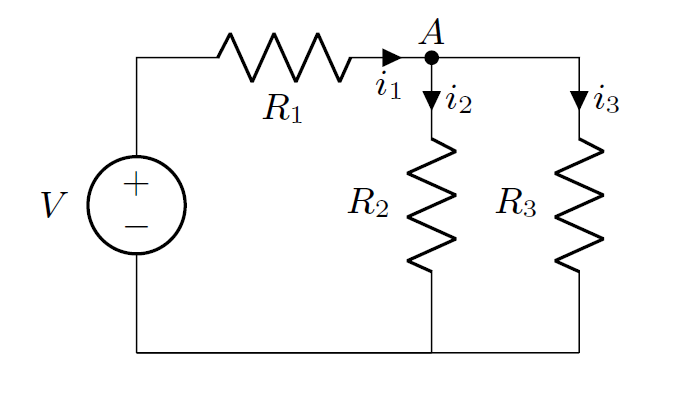
\includegraphics[width=0.6\linewidth]{Figuras/Ch02/fig2.PNG}}
	\begin{block}{Resolução}
		Primeira análise: $i_1 = i_2 + i_3$ \\
		Segunda análise: $i_1 - i_2 - i_3 = 0$ \\
		\begin{itemize}
			\item \textbf{Independente da abordagem escolhida, os resultados são equivalentes}.
		\end{itemize}
	\end{block}
}

\frame{
	\frametitle{Leis de Kirchhoff - LKT}
	\centerline{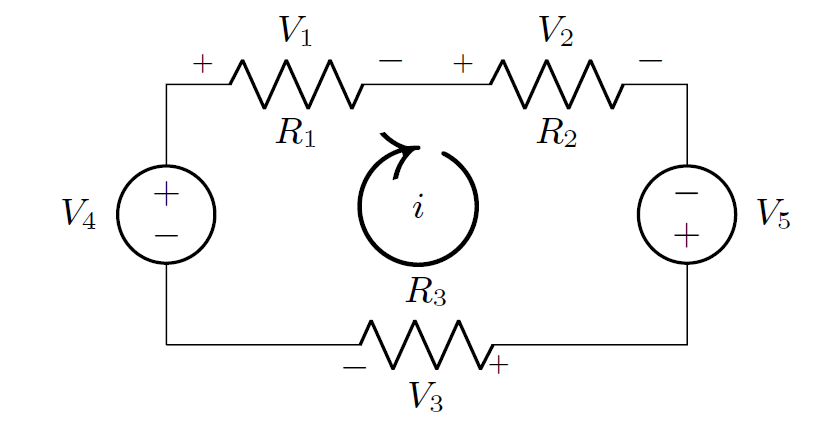
\includegraphics[width=0.7\linewidth]{Figuras/Ch02/fig3.PNG}}
	\begin{block}{Contextualização}
		A lei de Kirchhoff das tensões é aplicada nas malhas. Ela já foi usada no estudo dos
		circuitos de \textbf{resistores em série}, onde a soma das quedas de tensão nos resistores é igual à f.e.m. da fonte.
	\end{block}
}

\frame{
	\frametitle{Leis de Kirchhoff - LKT}
	\centerline{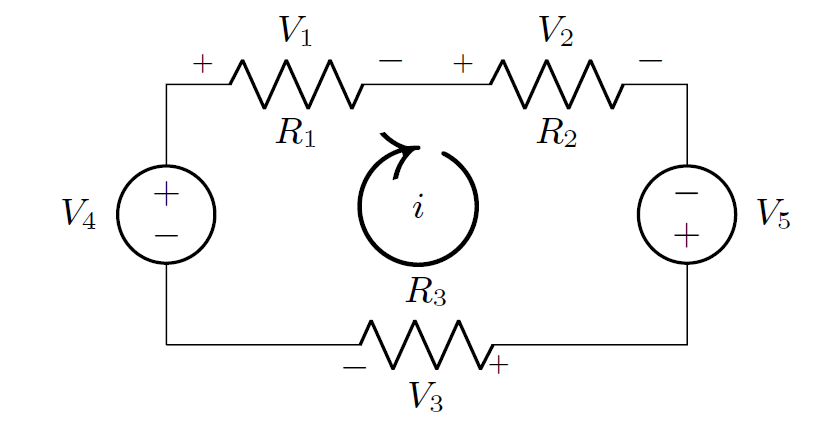
\includegraphics[width=0.6\linewidth]{Figuras/Ch02/fig3.PNG}}
	\begin{block}{Enunciado da 2a Lei de Kirchhoff}
		\textbf{``Em um percurso fechado, a soma algébrica das elevações de tensão é igual a soma algébrica das quedas de tensão."}
		$$\boxed{\sum_{i=1}^{n} V_{i_{\text{elevação}}} = \sum_{j=1}^{m} V_{j_{\text{queda}}}}$$
	\end{block}
}

\frame{
	\frametitle{Leis de Kirchhoff - LKT}
	\vspace{-0.3cm}
	\centerline{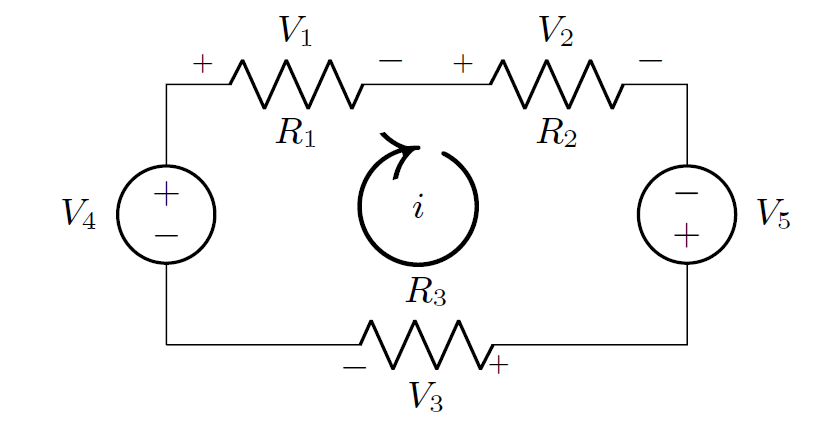
\includegraphics[width=0.6\linewidth]{Figuras/Ch02/fig3.PNG}}
	\begin{block}{Enunciado da 2a Lei de Kirchhoff - alternativo}
		\textbf{``A soma algébrica de todas as tensões em torno de um caminho fechado (ou malha) é zero"}. Consideramos que as \textbf{elevações} de tensão são \textbf{positivas} e as \textbf{quedas} de tensão são \textbf{negativas}.
		$$\boxed{\sum_{i=1}^{n} V_{i} = 0}$$
	\end{block}
}

\frame{
	\frametitle{Leis de Kirchhoff - LKT}
	\vspace{-0.3cm}
	\centerline{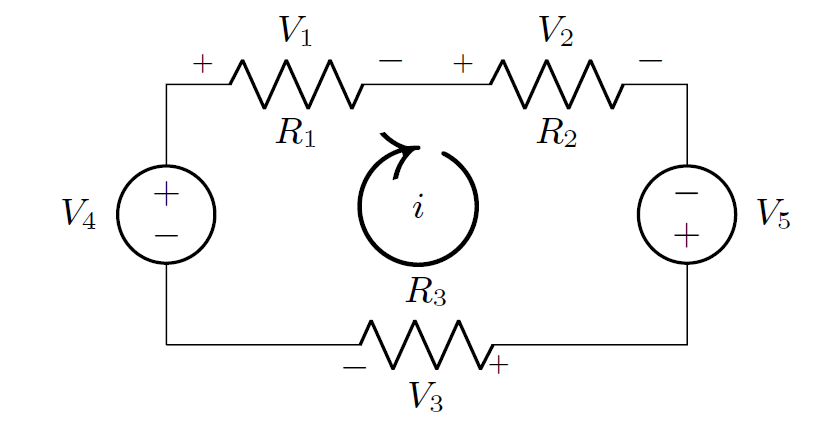
\includegraphics[width=0.7\linewidth]{Figuras/Ch02/fig3.PNG}}
	\begin{block}{Resolução - sentido horário da corrente}
		Primeira análise: $V_4 + V_5 = V_1 + V_2 + V_3$ \\
		Segunda análise: $V_4 - V_1 - V_2 + V_5 - V_3 = 0$ \\
		\begin{itemize}
			\item \textbf{Independente da abordagem escolhida, os resultados são equivalentes}.
		\end{itemize}
	\end{block}
}

\frame{
	\frametitle{Leis de Kirchhoff - LKT}
	\vspace{-0.3cm}
	\centerline{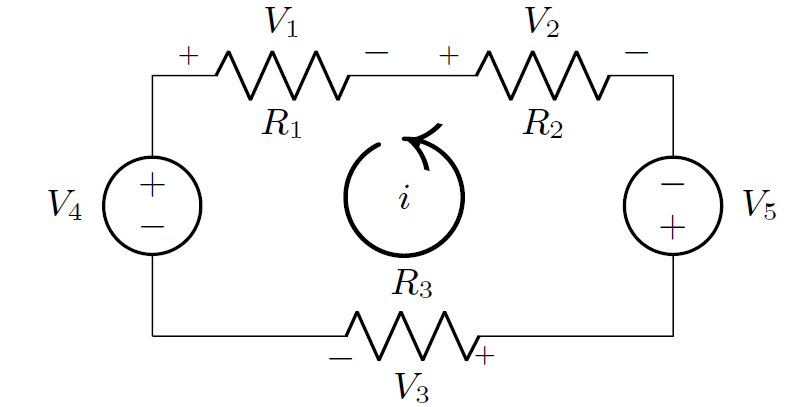
\includegraphics[width=0.7\linewidth]{Figuras/Ch02/fig4.PNG}}
	\begin{block}{Resolução - sentido anti-horário da corrente}
		Primeira análise: $V_2 + V_1 + V_3 = V_4 + V_5$ \\
		Segunda análise: $V_1 - V_4 + V_3 - V_5 + V_2 = 0$ \\
		\begin{itemize}
			\item \textbf{Independente da abordagem escolhida, os resultados são equivalentes}.
		\end{itemize}
	\end{block}
}

\section*{Exercícios}
\frame{
	\frametitle{Exercícios}
	\begin{block}{}
		01. Encontre $i_3$, $i_4$, $i_6$ e $i_7$.
		\vspace{0.1cm}
		\centerline{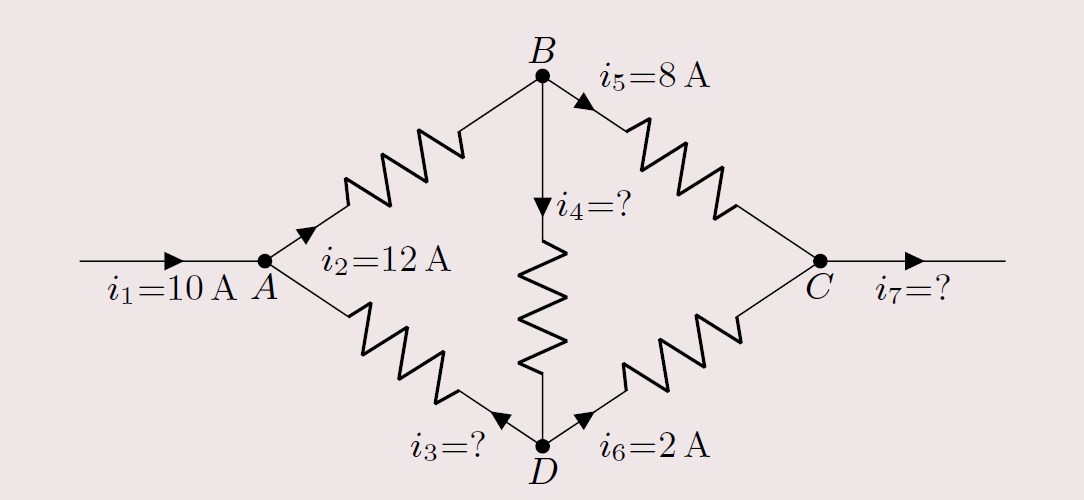
\includegraphics[width=0.9\linewidth]{Figuras/Ch02/fig5.PNG}}
	\end{block}
}

\section*{Exercícios}
\frame{
	\frametitle{Exercícios}
	\begin{block}{}
		02. Determine $V_1$ e $V_2$ no circuito abaixo.
		\centerline{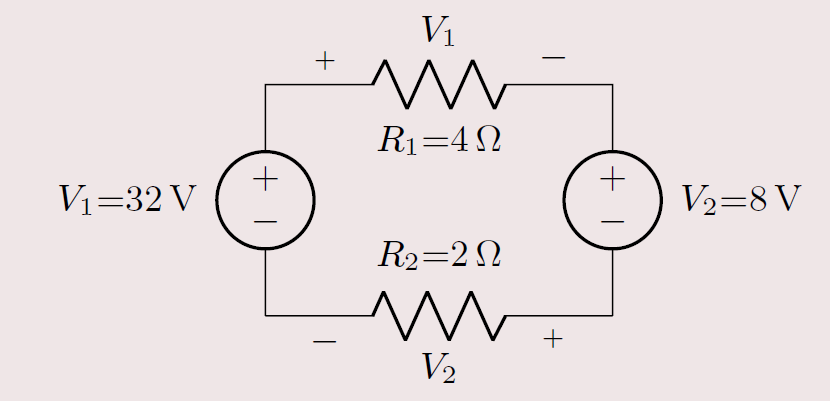
\includegraphics[width=0.8\linewidth]{Figuras/Ch02/fig6.PNG}}
	\end{block}
}

\section*{Referências}

\frame{
	\frametitle{Referências e Exercícios Complementares}
	\begin{itemize}
		\item ALEXANDRE, Charles K.; SADIKU, Matthew N. O. Fundamentos de Circuitos Elétricos. 5. ed. Porto Alegre: AMGH, 2013.
	\end{itemize}
	%\centering{\alert{Página 36 - \textbf{1.6.1 até 1.6.5, 1.6.17 até 1.6.19}}} \\
	\centering{\alert{Lista de exercícios 02}}
}



